\documentclass[12pt,fleqn]{article}
\usepackage[margin=1in,top=1in,bottom=1in]{geometry}
\usepackage{tikz}
\usepackage{mathtools}
\usepackage{longtable}
\usepackage{enumitem}
\usepackage{hyperref}
%\usepackage[dvips]{graphics}
%\usepackage{amssymb}
\usepackage{float}
%\usepackage[usenames]{xcolor}
%\usepackage{subfig}
\usepackage{booktabs}
\usepackage{subcaption}

\usepackage[normalem]{ulem}

\usepackage{multicol}
\usepackage{txfonts}
\usepackage{amsfonts}
\usepackage{natbib}
\usepackage{gb4e}
\usepackage[all]{xy}
\usepackage{rotating}
\usepackage{tipa}
\usepackage{multirow}
\usepackage{authblk}
\usepackage{url}
\usepackage{pdflscape}
\usepackage{rotating}
\usepackage{adjustbox}
\usepackage{array}


\def\bad{{\leavevmode\llap{*}}}
\def\marginal{{\leavevmode\llap{''}}}
\def\verymarginal{{\leavevmode\llap{''''}}}
\def\swmarginal{{\leavevmode\llap{4}}}
\def\infelic{{\leavevmode\llap{\#}}}

\definecolor{airforceblue}{rgb}{0.36, 0.54, 0.66}
%\definecolor{gray}{rgb}{0.36, 0.54, 0.66}

\definecolor{Pink}{RGB}{240,0,120}
\newcommand{\red}[1]{\textcolor{Pink}{#1}}
\newcommand{\jd}[1]{\textbf{\textcolor{Pink}{[jd: #1]}}}

\newcommand{\dashrule}[1][black]{%
  \color{#1}\rule[\dimexpr.5ex-.2pt]{4pt}{.4pt}\xleaders\hbox{\rule{4pt}{0pt}\rule[\dimexpr.5ex-.2pt]{4pt}{.4pt}}\hfill\kern0pt%
}

\setlength{\parindent}{2ex}
\setlength{\parskip}{.3ex}

\newcommand{\yi}{\'{\symbol{16}}}
\newcommand{\nasi}{\~{\symbol{16}}}
\newcommand{\hina}{h\nasi na}
\newcommand{\ina}{\nasi na}

\newcommand{\foc}{$_{\mbox{\small F}}$}

\hyphenation{par-ti-ci-pa-tion}

\setlength{\bibhang}{0.5in}
\setlength{\bibsep}{0mm}
\bibpunct[:]{(}{)}{,}{a}{}{,}

\newcommand{\6}{\mbox{$[\hspace*{-.6mm}[$}} 
\newcommand{\9}{\mbox{$]\hspace*{-.6mm}]$}}
\newcommand{\sem}[2]{\6#1\9$^{#2}$}
\renewcommand{\ni}{\~{\i}}

\newcommand{\citepos}[1]{\citeauthor{#1}'s \citeyear{#1}}
\newcommand{\citeposs}[1]{\citeauthor{#1}'s}
\newcommand{\citetpos}[1]{\citeauthor{#1}'s (\citeyear{#1})}

\newcolumntype{R}[2]{%
    >{\adjustbox{angle=#1,lap=\width-(#2)}\bgroup}%
    l%
    <{\egroup}%
}
\newcommand*\rot{\multicolumn{1}{R{90}{0em}}}% no optional argument here, please!

\newcommand{\jt}[1]{\textbf{\color{blue}JT: #1}}

\begin{document}

%Abstracts should fit two pages (letter size or A4 paper, 2.54cm or 1 inch margins on all sides, 12 point font, Times New Roman), with an additional third page used exclusively for the following elements: references (obligatory), large figures or tables,

\begin{center}
{\bf I have no idea if factivity is categorical. Did Mandelkern et al.\ 2020 discover that it is?}
\end{center}

\vspace*{-.5cm}

\noindent
This talk investigates the long-standing assumption that attitude predicates divide into factive and nonfactive ones (\citealt{kiparsky-kiparsky70,karttunen71b,heim92}, i.a.). This assumption was recently challenged by empirical investigations (e.g., \citealt*{demarneffe-etal-sub23,degen-tonhauser-language}), but \citealt*{mandelkern-etal2020} argued that the inference rating tasks used in these investigations are unsuitable to detect a categorical factivity distinction. This talk presents the results of an experiment that investigates factive and nonfactive predicates using the naturalness rating task advocated for in \citealt{mandelkern-etal2020}. The results again fail to support  a categorical factivity distinction, in line with \citealt{degen-tonhauser-language}.

\noindent
{\bf Introduction.} Attitude predicates have long been divided into factive and nonfactive ones based on whether the content of their clausal complement (CC) is presupposed (see references above): {\em know} is factive because interpreters infer that a speaker who utters (\ref{first}) with {\em know} believes that Julian dancing salsa is part of the common ground of the interlocutors (the CC ``projects''), whereas this inference does not arise with the variant of (\ref{first}) with nonfactive {\em think} (the CC ``does not project'').

\vspace*{-.2cm}
\begin{exe}
\ex\label{first} Ed: {\em ``Does Cole know/think that Julian dances salsa?''}
\end{exe}
\vspace*{-.2cm}

This classification of predicates was recently challenged based on empirical investigations (e.g., \citealt{demarneffe-etal-sub23,degen-tonhauser-language}). These investigations, which asked participants to draw inferences about the CC from examples like (\ref{first}), confirmed the long-standing intuition that the CCs of factive predicates are, generally, highly projective, but they also found i) that there is variability in how projective the CCs of factive predicates are, ii) that the CCs of factive predicates are not categorically more projective than those of nonfactive predicates, and iii) that the CCs of some factive predicates are less projective than that of nonfactive ones. These results were taken to suggest that ``there is little empirical support [...] for the assumed categorical distinction between factive and nonfactive predicates'' (\citealt[552]{degen-tonhauser-language}).

\citealt{mandelkern-etal2020} challenged this conclusion, arguing that gradient projection is an artifact of the inference task used, writing that ``inference tasks to some degree invite subjects to make the inference in question'' (p.498) and that ``we should think twice before embracing a notion of presupposition projection that is gradient based on results from inference tasks alone'' (p.497). They suggested that naturalness ratings of utterances with attitude predicates in explicit ignorance contexts (EICs), as in (\ref{second}), are more suitable to distinguishing the semantic presuppositions of factive predicates (hypothesized to be unnatural in EICs) from inferences that arise with nonfactive predicates ``for any of a variety of pragmatic reasons short of entailment or presupposition'' (p.497).

\vspace*{-.2cm}
\begin{exe}
\ex\label{second} Ed: \hspace*{-.2cm} {\em ``I have no idea if Julian dances salsa.}  \hspace*{-.1cm} {\em Does Cole know/think that Julian dances salsa?''}
\end{exe}
\vspace*{-.2cm}

\noindent
{\bf Methods.} To investigate \citepos{mandelkern-etal2020} claim that a categorical factivity distinction emerges from naturalness ratings in EICs, we collected such ratings for 20 (non)factive predicates. 

\noindent
\underline{Participants.} Data from 370 participants (ages: 19-80, mean: 40.7; 175 women, 185 men, 8 nonbinary, 2 undisclosed) were analyzed. Other data were excluded based on preregistered criteria.

\noindent
\underline{Materials.} Participants read two-sentence discourses consisting of an interrogative followed by a declarative, like (\ref{second}). In the target stimuli, the interrogatives combined the 20 factive and nonfactive predicates with the 20 complement clauses of \citealt{degen-tonhauser-openmind,degen-tonhauser-language}. The preceding declaratives implemented a three-level context condition: In the `explicit ignorance' context (\ref{second}), the declarative sentence conveyed the speaker's ignorance about the CC: If the CC is presupposed, global accommodation (taken to be default in \citealt{heim83,vds92}) is not possible and the discourse is expected to be unnatural; if the CC is not presupposed, the discourse is expected to be natural. In the other two context levels, the declarative denoted a fact relative to which the CC had a `low prior probability' (\ref{sample}a) or a `high prior probability' (\ref{sample}b); these contexts were normed in \citealt{degen-tonhauser-openmind}. Presupposition analyses (e.g., \citealt{heim83,vds92}) invariably predict global accommodation for presupposed CCs, that is, high naturalness ratings.

\vspace*{-.2cm}
\begin{exe}
\ex\label{sample}
\begin{xlist}
\ex Ed: {\em ``Julian is German. Did Cole discover that Julian dances salsa?''} \hspace*{-.2cm} \hfill [low prior prob.]
\ex Ed: {\em ``Julian is Cuban. Did Cole discover that Julian dances salsa?''} \hfill [high prior prob.]
\end{xlist}
\end{exe}
\vspace*{-.2cm}

In addition to the 1,200 target stimuli (20 predicates $\times$ 20 CCs $\times$ 3 contexts), the materials included six fillers: Four with hard triggers ({\em too, also, again},  {\em it-}clefts), expected to be unnatural in EICs (\citealt{simons01,abusch10}), and two with {\em stop} and {\em continue}, which \citealt{simons01} considers soft triggers (natural in explicit ignorance contexts), contrary to \citealt{mandelkern-etal2020} and \citealt{kalomoiros-schwarz2021}. The fillers were only presented in EICs.

\noindent
\underline{Procedure.} Participants rated the naturalness of ``[speaker's] question in this context'' on a slider from ``totally unnatural'' (coded 0) to ``totally natural'' (coded 1) for 30 stimuli: one target stimulus for each of the 20 predicates (each paired with a unique CC; 12 in EICs, and 4 each in low and high prior probability contexts), the six filler stimuli, and four acceptable control stimuli (used to identify participants not attending to the task). Trial order was randomized for each participant.
%\begin{exe}
%\ex Filler stimuli
%\begin{xlist}
%\ex I don't know if Ann plays any instrument. Does Ann play the flute, too?
%\ex I don't know if Svenja plays any sport. Does Svenja also play soccer?
%\ex I don't know if anyone was playing outside with the kids. Was it Jack who was playing outside with the kids?
%\ex I don't know if Stephen was ever in the habit of vaping. Has Stephen recently stopped vaping?
%\ex I don't know if John was ever reading ``Dune''. Has John recently continued reading ``Dune''?
%\ex I don't know if William was ever interested in history. Is William interested in history again?"
%\end{xlist}
%\end{exe}

%Finally, the experiment included 4 control stimuli, which were used to exclude participants not attending to the task. These were expected to be rated as natural/acceptable.

%Each participant saw a random set of 30 stimuli: Each set contained one target utterance for each of the 20 CCs (each paired with a unique clause-embedding predicates), the same 6 control stimuli, and the same 4  filler stimuli. 12 of the CCs were presented in the explicit ignorance context, 4 with a low prior probability fact, 4 with a high prior probability fact. Within-block trial order was randomized. After completing the experiment, participants filled out a short optional demographic survey. To encourage truthful responses, participants were told that they would be paid no matter what answers they gave in the survey.

%The experiment started off with four practice trials (2 natural, 2 unnatural; participants were given feedback on correct and incorrect answers).

\noindent
{\bf Results.} Contrary to \citepos{mandelkern-etal2020} claim, factives do not pattern alike, as shown in Fig.~\ref{fig:acc-by-expression}, which plots mean naturalness ratings in EICs by expression (colors: \color{orange}factives\color{black}, \color{gray}nonfactives\color{black}, hard triggers, \color{magenta}soft triggers\color{black}). Whereas the mean for {\em be annoyed} is at the level of the soft trigger {\em stop}, that of {\em know} is higher, and the means of {\em see, discover}, and {\em reveal} are as high as those of some nonfactive predicates. (These observations are confirmed by a linear mixed effects model, shown in the talk.) Thus, in line with \citealt{degen-tonhauser-language}, there is no empirical evidence for a categorical distinction between factive and non-factive predicates. (The talk also discusses that the results do not align with assumptions about hard and soft triggers; \citealt{simons01,abusch10}.)

Contrary to the predictions of presupposition analyses, the naturalness ratings of the purportedly factive predicates are sensitive to the low vs.\ high prior probability context manipulation. As shown in Fig.~\ref{fig:acc-by-context}, which plots mean naturalness ratings by context and expression, the mean naturalness ratings are higher in the high prior probability context than in the low one. This context-sensitivity, which is also observed for the nonfactive predicates (except {\em pretend}; model details provided in talk), replicates \citepos{degen-tonhauser-openmind} results, obtained using an inference rating task.

\noindent
{\bf Methodological and theoretical implications.} The recent challenge to the categorical factivity distinction by \citealt{degen-tonhauser-language} is not addressed by collecting naturalness ratings in EICs instead of inference ratings. And while naturalness ratings in EICs may provide insight into the meanings of attitude predicates, the interpretation of the results depends on the presumed linking function (as discussed in the talk; see, e.g., \citealt{sprouse2018}). The very low mean naturalness rating for {\em be annoyed} in EICs could, for instance, be due not to a semantic presupposition (see also \citealt{karttunen2016}) but because the CC is not-at-issue, contrary to what is suggested by the EIC.

Contemporary presupposition analyses (e.g., \citealt{heim83,vds92,abrusan2011,karttunen2016,simons-etal2017}) predict neither the heterogeneity of the naturalness ratings of factive predicates nor their sensitivity to the prior probability of the CC. These results, which mirror those based on inference ratings, suggest that projection analyses must incorporate more fine-grained distinctions between attitude predicates and the systematic effect of prior probabilities.

\newpage

\begin{figure}[h!]
\centering
\caption{\small{Mean naturalness rating in explicit ignorance context by expression (\color{orange}factive\color{black}, \color{gray}nonfactive\color{black}, \color{magenta} soft trigger\color{black}, \color{black}hard trigger\color{black}). Error bars indicate 95\% bootstrapped CIs. Violin plots indicate kernel probability density of participants' ratings.}}\label{fig:acc-by-expression}
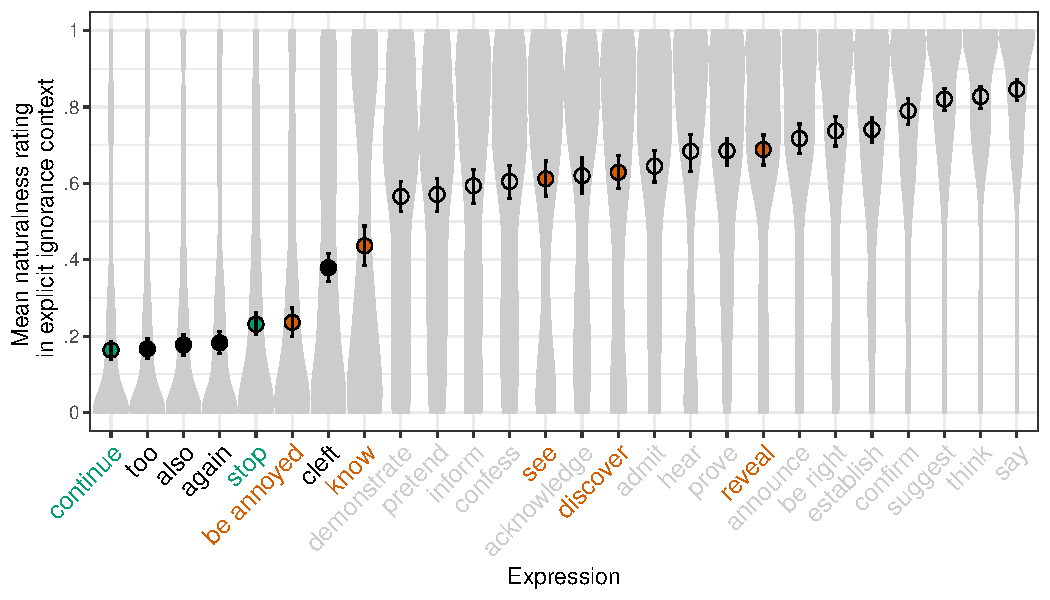
\includegraphics[width=.9\textwidth]{../../results/main/13explicitIgnorance/graphs/explicit-ignorance-naturalness-by-predicate}
\end{figure}

\vspace*{-1cm}

\begin{figure}[h!]
\centering
\caption{\small{Mean naturalness rating by context and predicate (\fcolorbox{black}{orange}{factive}, \fcolorbox{black}{lightgray}{nonfactive}); predicates ordered as in Fig.~\ref{fig:acc-by-expression}. Error bars indicate 95\% bootstrapped CIs. Violin plots indicate kernel probability density of participants' ratings}.}\label{fig:acc-by-context}
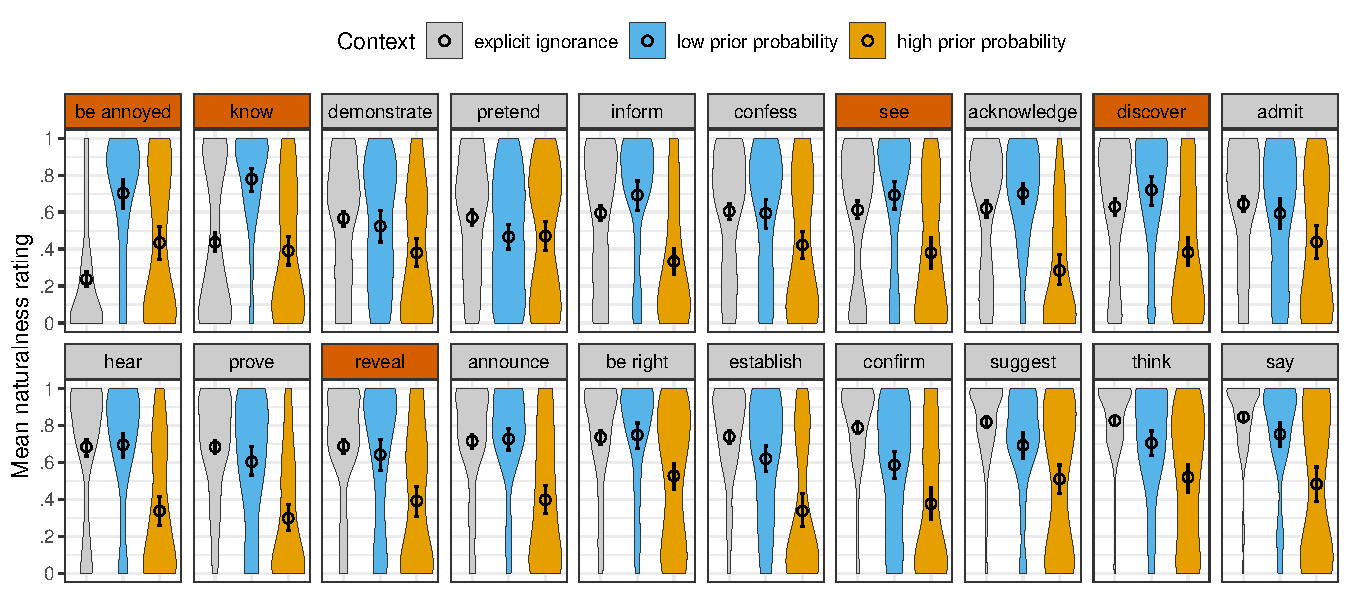
\includegraphics[width=\textwidth]{../../results/main/13explicitIgnorance/graphs/ORDER-by-LANGUAGE-naturalness-by-context-and-predicate}
\end{figure}

\vspace*{-.7cm}

\renewcommand\bibsection{\subsubsection*{\refname}}
\begin{tiny}
\bibliographystyle{cslipubs-natbib}
\bibliography{/Users/tonhauser.1/Documents/bibliography}
\end{tiny}


 
\end{document}

